In this chapter, we first introduce the quasi-2D Coulomb systems, along with the mathematical notations used throughout this thesis.
Then we revisit the Ewald summation method for doubly periodic lattice sums and its extension to dielectric-confined systems through combination with the image charge method, as well as its reformulation.
Finally we will introduce the random batch Ewald (RBE) method, which is a powerful method to accelerate the computation of the electrostatic energy.

\section{Quasi-2D Coulomb systems}

Quasi-2D systems are three-dimensional models characterized by double periodicity in the $xy$ dimensions and confinement by planar dielectric interfaces along the $z$-axis.
The characteristic length scale in the non-periodic direction is often significantly smaller than that in the periodic directions. 
In what follows, we present the mathematical formulation of the model.

Consider two parallel dielectric interfaces positioned at $z=0$ and $z=H$, dividing the entire 3D space $\mathbb{R}^3$ into three distinct layers. 
From top to bottom, these layers are denoted as $\Omega_{\text{u}}$, $\Omega_{\text{c}}$ and $\Omega_{\text{d}}$, respectively. 
The central simulation cell $\Omega\in\Omega_{\text{c}}$ has side lengths~$\bm{L}=(L_x, L_y, H)$ and contains $N$ particles located at $\{\V{r}_i\}_{i=1}^{N}$ with charges $\{q_i\}_{i=1}^{N}$. 
The total charge neutrality condition is assumed, i.e., $\sum_{i=1}^{N}q_i=0$. The dielectric permittivity is a piecewise constant function, defined as:
\begin{equation}\label{eq:sanwich}
    \eps(\V{r})=\left\{
        \begin{array}{ll}
        \epsilon_{\mrm{u}}, &\, {\V{r} \in \Omega_{\mrm{u}}},\\
        \epsilon_{\mrm{c}}, &\, {\V{r} \in \Omega_{\mrm{c}}},\\
        \epsilon_{\mrm{d}}, & \,{\V{r} \in \Omega_{\mrm{d}}},
    \end{array} \right.
\end{equation}
where~$\eps_{\T u}$,~$\eps_{\T c}$ and~$\eps_{\T d}$ are all positive constants, whose specific values depend on materials properties inside each layer. 
An illustration of the quasi-2D charged system is shown in Fig.~\ref{fig:box}.

\begin{figure}[htbp]
    \centering
    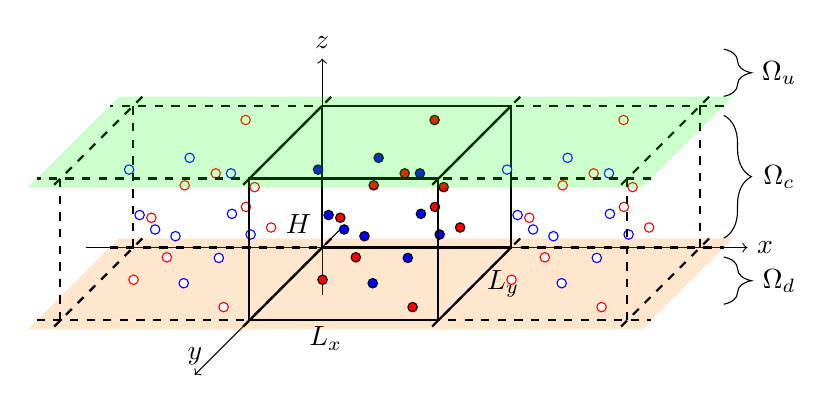
\begin{tikzpicture}[scale=0.6]

        \draw[->] (-5, 0, 0) -- (9, 0, 0) node[right] {$x$}; % x-axis
        \draw[->] (0, -1, 0) -- (0, 4, 0) node[above] {$z$}; % y-axis
        \draw[->] (0, 0, -1) -- (0, 0, 7) node[above] {$y$}; % z-axis

        \fill[orange, opacity=0.2] (-4.5, 0, -0.5) -- (8.5, 0, -0.5) -- (8.5, 0, 4.5) -- (-4.5, 0, 4.5);
        % \fill[orange, opacity=0.2] (-4.5, 0, 4.5) -- (8.5, 0, 4.5) -- (8.5, -0.5, 4.5) -- (-4.5, -0.5, 4.5);
        % \fill[orange, opacity=0.2] (8.5, 0, -0.5) -- (8.5, 0, 4.5) -- (8.5, -0.5, 4.5) -- (8.5, -0.5, -0.5);

        \draw[thick] (0, 0, 0) -- (4, 0, 0) -- (4, 3, 0) -- (0, 3, 0) -- cycle; % Bottom face

        \foreach \x/\y/\z in {1.1681915835663497/0.4784386449304706/3.0114784670813646, 1.37700874310584/0.4564910752408716/1.723302872827872, 3.730994750135867/1.2345031904085388/2.103105645365449, 1.827895374334192/2.07357017874381/3.746941345635766, 3.066558538444058/1.5385426337573604/1.7619877149348904, 1.323901301301564/1.5495075401772844/0.6031052215686215, 3.756938726146066/2.4640736386255653/3.077635065930065, 2.8772957887165047/2.6997418470234025/2.9329762207627343, 3.2340462748359378/0.05840416805411408/3.426026606528974, 2.6025039709080175/2.9218252913656833/0.57717965442315666} {
            \draw[fill=red] (\x, \y, \z) circle (0.1);
        }

        \foreach \x/\y/\z in {2.6498617350978773/2.150049613814989/1.5048602780413822, 3.089169032276023/1.0562600341829351/3.3127362964215057, 2.5980246280095605/0.7722521776014004/3.9662770148938087, 1.1349256153410514/2.870534190907561/3.169316637530182, 3.1201708293697656/0.9091412698002154/1.6441954803083996, 1.9206578784987878/2.6240285163641914/1.8820001242058, 2.21640094284661/0.839090054913301/0.3248449650128413, 1.7055625414319642/1.0502926700849304/2.1025386222981464, 1.9224549177172139/1.8402480747416887/3.7853267350243893, 0.6942437596034523/1.2454445897320752/1.4473021778716602} {
            \draw[fill=blue] (\x, \y, \z) circle (0.1);
        }

        \foreach \dx/\dy in {-4/0, 4/0} {
            \foreach \x/\y/\z in {1.1681915835663497/0.4784386449304706/3.0114784670813646, 1.37700874310584/0.4564910752408716/1.723302872827872, 3.730994750135867/1.2345031904085388/2.103105645365449, 1.827895374334192/2.07357017874381/3.746941345635766, 3.066558538444058/1.5385426337573604/1.7619877149348904, 1.323901301301564/1.5495075401772844/0.6031052215686215, 3.756938726146066/2.4640736386255653/3.077635065930065, 2.8772957887165047/2.6997418470234025/2.9329762207627343, 3.2340462748359378/0.05840416805411408/3.426026606528974, 2.6025039709080175/2.9218252913656833/0.57717965442315666} {
            \draw[draw=red, fill=white] (\x + \dx, \y + \dy, \z) circle (0.1);
        }

            \foreach \x/\y/\z in {2.6498617350978773/2.150049613814989/1.5048602780413822, 3.089169032276023/1.0562600341829351/3.3127362964215057, 2.5980246280095605/0.7722521776014004/3.9662770148938087, 1.1349256153410514/2.870534190907561/3.169316637530182, 3.1201708293697656/0.9091412698002154/1.6441954803083996, 1.9206578784987878/2.6240285163641914/1.8820001242058, 2.21640094284661/0.839090054913301/0.3248449650128413, 1.7055625414319642/1.0502926700849304/2.1025386222981464, 1.9224549177172139/1.8402480747416887/3.7853267350243893, 0.6942437596034523/1.2454445897320752/1.4473021778716602} {
                \draw[draw=blue, fill=white] (\x + \dx, \y + \dy, \z) circle (0.1);
            }
        }

        
        \draw[thick] (0, 0, 4) -- (4, 0, 4) -- (4, 3, 4) -- (0, 3, 4) -- cycle; % Top face
        \draw[thick] (0, 0, 0) -- (0, 0, 4); % Front left
        \draw[thick] (4, 0, 0) -- (4, 0, 4); % Front right
        \draw[thick] (4, 3, 0) -- (4, 3, 4); % Back right
        \draw[thick] (0, 3, 0) -- (0, 3, 4); % Back left

        % Draw dashed boxes for all 8 neighboring boxes
        \foreach \dx/\dy in {-4/0, 4/0} {
            \draw[thick, dashed] (\dx - 0.5, 0, \dy) -- (4.5 + \dx, 0, \dy);
            \draw[thick, dashed] (4 + \dx, 0, \dy) -- (4 + \dx, 3, \dy);
            \draw[thick, dashed] (4.5 + \dx, 3, \dy) -- (\dx - 0.5, 3, \dy);
            \draw[thick, dashed] (\dx, 0, \dy) -- (\dx, 3, \dy);

            \draw[thick, dashed] (\dx - 0.5, 0, 4 + \dy) -- (4.5 + \dx, 0, 4 + \dy);
            \draw[thick, dashed] (4 + \dx, 0, 4 + \dy) -- (4 + \dx, 3, 4 + \dy);
            \draw[thick, dashed] (4.5 + \dx, 3, 4 + \dy) -- (\dx - 0.5, 3, 4 + \dy);
            \draw[thick, dashed] (\dx, 0, 4 + \dy) -- (\dx, 3, 4 + \dy);

            \draw[thick, dashed] (\dx, 0, \dy - 0.5) -- (\dx, 0, 4.5 + \dy); % Front left
            \draw[thick, dashed] (4 + \dx, 0, \dy - 0.5) -- (4 + \dx, 0, 4.5 + \dy); % Front right
            \draw[thick, dashed] (4 + \dx, 3, \dy - 0.5) -- (4 + \dx, 3, 4.5 + \dy); % Back right
            \draw[thick, dashed] (\dx, 3, \dy - 0.5) -- (\dx, 3, 4.5 + \dy); % Back left
        }

        \fill[green, opacity=0.2] (-4.5, 3, -0.5) -- (8.5, 3, -0.5) -- (8.5, 3, 4.5) -- (-4.5, 3, 4.5) -- cycle;
        % \fill[green, opacity=0.2] (-4.5, 3, -0.5) -- (8.5, 3, -0.5) -- (8.5, 3.5, -0.5) -- (-4.5, 3.5, -0.5) -- cycle;
        % \fill[green, opacity=0.2] (-4.5, 3, -0.5) -- (-4.5, 3, 4.5) -- (-4.5, 3.5, 4.5) -- (-4.5, 3.5, -0.5) -- cycle;


        \node at (2, 0, 5) {$L_x$};
        \node at (4.6, 0, 2) {$L_y$};
        \node at (-0.5, 0.5, 0) {$H$};

        \draw[decorate, decoration={brace, amplitude=10pt, mirror}] (8.5, 0.2, 0) -- (8.5, 2.8, 0) node[midway,xshift=20] {$\Omega_{\mrm{c}}$};
        \draw[decorate, decoration={brace, amplitude=10pt, mirror}] (8.5, 3.2, 0) -- (8.5, 4.2, 0) node[midway,xshift=20] {$\Omega_{\mrm{u}}$};
        \draw[decorate, decoration={brace, amplitude=10pt, mirror}] (8.5, -1.2, 0) -- (8.5, -0.2, 0) node[midway,xshift=20] {$\Omega_{\mrm{d}}$};

    \end{tikzpicture}
    \caption{
        A schematic of the quasi-2D charged system.
        The filled circles represent the charged particles confined in the central simulation box, and the empty circles represent the periodic replicas in $xy$ plane.
        The green and orange regions represent the sharp dielectric interfaces $\partial \Omega_c \cap \partial \Omega_{u}$ and $\partial \Omega_c \cap \partial \Omega_{d}$ , respectively.
        As the system is doubly periodic in both $xy$ directions, here only the periodicity in~$x$ is sketched for clarity.
    }
    \label{fig:box}
\end{figure}

\subsection{Homogeneous Quasi-2D Systems}

We first introduce the case where the dielectric constants are equal throughout the system, i.e.,~$\eps_{\mrm{u}} = \eps_{\mrm{d}} = \eps_{\mrm{c}}$. For simplicity, we set~$\eps_{\mrm{u}} = \eps_{\mrm{d}} = \eps_{\mrm{c}} = 1$.
The electrostatic potential $\phi(\V r)$ for such systems then is governed by the following Poisson's equation with doubly periodic boundary conditions (DPBCs):
\begin{equation}\label{eq::Poisson}
	-\Delta\phi(\bm{r}) = 4\pi g(\bm{r}), \quad \text{with} \quad g(\bm{r})= \sum_{\V{m}}\sum_{j=1}^{N}q_{j}\delta(\bm{r}-\bm{r}_{j}+\bm{\mathcal{M}}),%\quad \lim_{z\rightarrow \infty}\nabla_{z}\phi(\bm{r})=0,
\end{equation}
% where $\bm{m}=(m_x,m_y,0)$ with $(m_x,m_y)\in\mathbb{Z}^2$, $\V{L}=(L_x,L_y,L_z)$, and $\bm{\mathcal{M}} := \bm{m}\circ\bm{L}$.
where $\bm{m}=(m_x,m_y) \in\mathbb{Z}^2$, and $\bm{\mathcal{M}} := (m_x L_x, m_y L_y, 0)$.
The solution to Eq.~\eqref{eq::Poisson} is doubly-periodic $\phi(\bm{r})=\phi(\bm{r} + \bm{\mathcal{M}})$ and unique up to a linear function in $z$. The uniqueness will be satisfied by incorporating a suitable boundary condition as $z\to\pm\infty$.

In many practical situations, the potential is defined via the following Coulomb summation formulation,
\begin{equation}\label{eq::pairssum}
	\phi(\bm{r})=\sum_{\V{m}}\sum_{j=1}^{N}\frac{q_{j}}{|\bm{r}-\bm{r}_{j} + \bm{\mathcal{M}}|}\;,
\end{equation}
where one should notice that the potential is singular when $\bm{r}=\bm{r}_{j}$ and $\bm{m}=\bm{0}$, the singularity comes from the Dirac delta source. 
It is important to note that Eq.~\eqref{eq::pairssum} is not well defined without specifying the shape of summation region~\cite{de1980simulation,smith2008electrostatic} and the total charge neutrality condition. 
We construct copies $\Omega(\bm{m})$ of the simulation domain by $\Omega(\bm{m})=\{\bm{r}|\bm{r}-\bm{\mathcal{M}}\in\Omega\}$. One has $\Omega(\bm{0})\equiv\Omega$ and a copied domain $\Omega(\bm{m})$ contains $N$ charges at $\bm{r}_j+\bm{\mathcal{M}}$. 
% Next, we define a summation shape $\mathcal{S}$ which contains the origin $\bm{m}=\bm{0}$ and has surface $f_{\mathcal{S}}=0$. 
Next, we define a summation shape $\mathcal{S} \subset \mathbb{R}^2$ which contains the origin.
% and has surface $f_{\mathcal{S}}(\V{r}) = 0$.
We consider a lattice $\Lambda(\mathcal{S},R)=\{\Omega(\bm{m})|\bm{m}/R\in\mathcal{S}\}$ with $R\in\mathbb{R}$ be a truncation parameter. 
Given these notations, Theorem \ref{order} clarifies the necessary conditions to guarantee absolute convergence of the series.

\begin{thm} \label{order}
    The summation in Eq.~\eqref{eq::pairssum} truncated within region $\Lambda(\mathcal{S},R)$ is absolutely convergent as~$R \to \infty$ if (1) the shape $\mathcal{S}$ is symmetric around the origin (meaning that if $\bm{m} / R \in \mathcal{S}$, then $- \bm{m}/ R \in \mathcal{S}$);and (2) the system within the central box is charge neutral, i.e.,~$\sum_{j = 1}^N q_j = 0$.
\end{thm}

\begin{proof}
	By the Taylor expansion, one has for large $|\bm{m}|$
	\begin{equation}\label{eq::3}
		\frac{1}{|\bm{r} + \bm{\mathcal{M}}|} = \frac{1}{|\bm{\mathcal{M}}|} - \frac{\bm{r} \cdot \bm{\mathcal{M}}}{|\bm{\mathcal{M}}|^3} + \mathcal{O} \left(\frac{1}{|\mathcal{\sM M}|^3}\right)\;.
	\end{equation}
	In the right-hand side of Eq.~\eqref{eq::3}, the second term is odd with respect to $\V{m}$ and thus sums to zero due to the symmetry of $\mathcal{S}$. The last $\mathcal{O}(|\V{\mathcal{M}}|^{-3})$ term is absolutely convergent as $R\rightarrow \infty$. Therefore, it is sufficient to analyze the convergence behavior of the expression:
	\begin{equation}\label{eq::4}
		% J=\lim_{R\rightarrow\infty}\sum_{\bm{\mathcal{M}} \in \mathcal{S}}\frac{1}{|\bm{\mathcal{M}}|}\sum_{j=1}^{N}q_{j}.
        J=\lim_{R\rightarrow\infty}\sum_{\bm{m}/ R \in \mathcal{S}}\frac{1}{|\bm{\mathcal{M}}|}\sum_{j=1}^{N}q_{j}.
	\end{equation}
	Eq.~\eqref{eq::4} can be viewed as a Riemann sum multiplied by the total net charges. If the charge neutrality condition is satisfied, i.e., $\sum_{j=1}^{N}q_{j}=0$, then $J$ vanishes and the series summation of $\phi$ in Eq.~\eqref{eq::pairssum} is absolutely convergent. 
	If the charge neutrality condition is violated, the Riemann sum can be approximated as an integral, $J\sim 2\pi (L_xL_y)^{-1} R\sum_{j=1}^{N}q_{j}$, which diverges as $R\rightarrow \infty$. This implies that the total charge neutrality condition is a necessary requirement for the existence of $\phi(\bm{r})$ in Eq.~\eqref{eq::pairssum}.
\end{proof}
%It is remarked that, for fully-periodic systems, the pairwise Coulomb summation is conditionally convergent\cite{de1980simulation}, meaning that the series summation result depends on the specific shape of summation region.

In practice, a common choice is to choose the spherical/circular shape of summation region centered at the origin with unit radius; i.e., the sum is taken over $\abs{\V m}=0, 1, 2\ldots, R$ in ascending order, where $R$ is the truncation parameter.
As long as Eq.~\eqref{eq::pairssum} is well defined, Proposition~\ref{prop::boundary} establishes a precise relationship between Eq.~\eqref{eq::pairssum} and the solution to Poisson's equation Eq.~\eqref{eq::Poisson} given a properly chosen boundary condition as $z\to\infty$.

\begin{prop}\label{prop::boundary}
	If the the series summation of $\phi(\bm{r})$ in Eq.~\eqref{eq::pairssum} satisfies both conditions stated in Theorem~\ref{order}, then it is a unique solution to Poisson's equation Eq.~\eqref{eq::Poisson} given the far-field boundary condition
	\begin{equation}\label{eq::boundary1}
		\lim_{z \to \pm \infty} \phi(\bm{r}) = \pm \frac{2\pi}{L_x L_y} \sum_{j=1}^{N} q_{j} z_{j}\;.
	\end{equation}
\end{prop}

\begin{proof}
	Let~$\bm{\rho}=(x,y)$ and $\bm{k}=(k_x, k_y)$ denote the periodic dimensions of position and Fourier frequency, respectively, where $\bm{\rho}\in\mathcal{R}^2$ and $\bm{k}\in\mathcal{K}^2$ with
	\begin{equation}
		\mathcal{R}^2:=\{\bm{\rho}\in[0,L_x]\times [0,L_y]\},\quad \text{and}\quad \mathcal{K}^2:=\left\{\bm{k}\in\frac{2\pi}{L_x}\mathbb{Z}\times \frac{2\pi}{L_y}\mathbb{Z}\right\}\;.
	\end{equation} 
	The Poisson's summation formula~(see~\ref{app::Fourier}) indicates 
	\begin{equation}\label{eq::9}
		% \sum_{\V{m}} \frac{q_{0}}{|\bm{r}-\bm{r}_{0} + \bm{\mathcal{M}}|} = \frac{2 \pi}{L_x L_y} q_0 \sum_{\bm{k}} \frac{e^{-k \abs{z - z_0}}}{k} e^{- \m{i} \bm{k} \cdot (\bm{\rho} - \bm{\rho_0})}\;,
		\sum_{\V{m}} \sum_{j = 1}^N \frac{q_{j}}{|\bm{r}-\bm{r}_{j} + \bm{\mathcal{M}}|} =  \sum_{j = 1}^N q_j \left[ \frac{2 \pi}{L_x L_y} \sum_{\bm{k} \neq \bm{0}} \frac{e^{-k \abs{z - z_j}}}{k} e^{- \m{i} \bm{k} \cdot (\bm{\rho} - \bm{\rho_j})} + \phi_{\bm{0}}(z-z_j)\right]\;,
	\end{equation}
	where~$k=|\bm{k}|$ and 
	\begin{equation}\label{eq::91}
		\phi_{\bm{0}}(z-z_j) = \frac{2\pi}{L_x L_y} \int_{0}^\infty \frac{ \rho}{\sqrt{\rho^2 + |z - z_j|^2}} d\rho
	\end{equation}
	represents the~$\bm{k}=\bm{0}$ term. Note that Eq.~\eqref{eq::91} is equivalent to a uniformly charged infinite plane in the real space. 
	As~$z \to \infty$, all~$\bm{k} \neq \bm{0}$ modes vanish, so that 
	\begin{equation}
		\lim_{z \to \pm \infty} \phi(\bm{r})=\lim_{z \to \pm \infty}\sum_{j=1}^{N}q_j\phi_{\bm{0}}(z-z_j).
	\end{equation}
	%\begin{equation}
	%    \begin{split}
		%         \lim_{z \to \pm \infty} \phi(\bm{r})
		%         &= \lim_{z \to \pm \infty} \sum_{j = 1}^N \frac{q_j}{L_x L_y} \int_{0}^\infty \frac{2\pi \rho}{\sqrt{\rho^2 + |z - z_j|^2}} d\rho. \\
		%     \end{split}
	%\end{equation}
	One can then integrate out Eq.~\eqref{eq::91} and arrives at
	\begin{equation}\label{eq::boundary2}
		\lim_{z \to \pm \infty} \phi(\bm{r}) = -\lim_{z \to \pm \infty} \frac{2\pi}{L_x L_y} \sum_{j = 1}^N q_j \abs{z - z_j}.
	\end{equation}
	Finally, the charge neutrality condition results in Eq.~\eqref{eq::boundary1}. 
 
Eq.~\eqref{eq::boundary1} indicates that $\lim\limits_{z \to \pm \infty} \phi(\bm{r})$ is a finite constant, and thus can be regarded as a properly chosen Dirichlet-type boundary condition at $z\rightarrow\pm\infty$~\cite{lindbo2012fast}. 
Next, we study the uniqueness of the solution of Poisson's equation under DPBCs and Eq.~\eqref{eq::boundary1}. Suppose there exists two solutions $\phi_1(\bm{r})$ and $\phi_2(\bm{r})$,
let $u(\bm{r}):=\phi_1(\bm{r})-\phi_2(\bm{r})$ be the difference between two solutions, and $\mathcal{B}=\mathcal{R}^2\times\mathbb{R}$ be a tubular cell that extends to infinity in the $z$-direction. By Green's first identity, we have 
\begin{equation}
0=\int_{\mathcal{B}}u\Delta ud\bm{r}=\int_{\mathcal{B}}\nabla\cdot(u\nabla u)-(\nabla u)^2d\bm{r}=\int_{\partial\mathcal{B}}u\nabla u\cdot d\bm{S}-\int_{\mathcal{B}}\left(\nabla u\right)^2d\bm{r}.
\end{equation}
The boundary term in the RHS cancels by periodicity in the $xy$-plane as well as $\lim\limits_{z\rightarrow\pm\infty}u(\bm{r})=0$, hence $\nabla u(\bm{r})\equiv \bm{0}$ in $\mathcal{B}$. Accordingly, we have $u(\bm{r})\equiv 0$, which ensures the uniqueness of the solution.
  
%It has been proved that with the doubly periodic boundary conditions, the solution to Poisson's equation Eq.~\eqref{eq::Poisson} is unique up to a piecewise linear function in $z$~\cite{lindbo2012fast, barnett2018unified}, so that the boundary condition Eq.~\eqref{eq::boundary1} is sufficient to determine the unique solution to Eq.~\eqref{eq::Poisson}.
\end{proof}

For such a well-defined quasi-2D Coulomb system, the electrostatic \emph{interaction energy} $U$ is given by
% \begin{equation}\label{eq::intenergy}
	%     U(\bm{r}_1, \ldots,\bm{r}_N) = W(\bm{r}_1, \ldots,\bm{r}_N) - \sum_{i=1}^N W(\bm{r}_i)\;,
	% \end{equation}
% where $W(\bm{r}_1, \ldots,\bm{r}_N)$ is the electrostatic total energy for a $N$-particle system, and $W(\mathbf{r}_i)$ the total energy for a single-particle system. 
% Due to the uniform background assumption, the single particle energy $W(\mathbf{r}_i)$ is translational invariant. 
% Substituting Eq.~\eqref{eq::pairssum} into~\eqref{eq::intenergy}, one has
\begin{equation} \label{eq::U_pair}
	U(\bm{r}_1, \ldots,\bm{r}_N)= \frac{1}{2} \sum_{\V{m}} \sum_{i=1}^{N} \sum_{j=1}^N {}^\prime \frac{q_i q_j} {|\bm{r}_{i}-\bm{r}_{j} + \bm{\mathcal{M}}|}\;,
\end{equation}
where the notation ``$\prime$'' represents that the~$i = j$ case is excluded when~$\bm{m} = \bm{0}$.
The corresponding force on each particle is $\bm{F}^i=-\nabla_{\bm{r}_{i}} U$, for $i=1,2,\ldots, N$.
It is remarked that, though the quasi-2D Coulomb summation is absolutely convergent, due to the long-range nature of Coulomb interaction, directly truncating the series for computing energy or force will lead to slow convergence with a complexity of $\mathcal O(N^2)$.


\subsection{Dielectric Confined Quasi-2D Systems}

Then we consider the case where the dielectric constants are different in the upper and lower regions, i.e.~$\eps_{\mrm{u}}, \eps_{\mrm{d}} \neq \eps_{\mrm{c}}$.
We assume that the interaction energy can be represented as
\begin{equation}\label{eq:U_direct}
    U = \frac{1}{2} \sum_{\V{m}} {}^\prime \sum_{i=1}^{N}\sum_{j=1}^{N} q_i q_j G(\V{r}_i,~\V{r}_j + \bm{\mathcal{M}})\;,
\end{equation}
where the Green's function $G(\V{r},~\V{r}^\prime)$, which describes the electrostatic response at any target location $\V r\in\mathbb{R}^3$ due to a point source charge located at $\V{r}^\prime\in\Omega$, satisfying Poisson's equation with dielectric interface conditions:
\begin{equation}
    \left\{
    \begin{array}{ll}
        - \grad_{\V{r}} \left[ \eps(\V{r}) \grad_{\V{r}} G(\V{r},~\V{r}^\prime) \right] = \d (\V{r} - \V{r}^\prime) & r \in \mathbb{R}^3 \;, \\
        G(\V{r},~\V{r}^\prime) |_{-} = G(\V{r},~\V{r}^\prime) |_{+} & \text{on}~\partial\Omega_{\T c}\;, \\
        \eps_{\T c} G_{\bm{n}}(\V{r},~\V{r}^\prime) |_{-} = \eps_{\T u}  G_{\bm{n}}(\V{r},~\V{r}^\prime) |_{+} & \text{on}~\partial \Omega_{\T c} \cap \partial \Omega_{\T u}\;, \\
        \eps_{\T c} G_{\bm{n}}(\V{r},~\V{r}^\prime) |_{+} = \eps_{\T {d}} G_{\bm{n}}(\V{r},~\V{r}^\prime) |_{-} & \text{on}~\partial \Omega_{\T c} \cap \partial \Omega_{\T d}\;, \\
        G(\V{r},~\V{r}^\prime) \to 0 & \text{as}~r \to \infty\;,
    \end{array}
    \right.
    \label{eq:Poisson_G}
\end{equation}
where $G_{\bm{n}}$ represents the normal derivative of $G$ at planar interfaces, and the subscripts ``$+$/$-$'' denote exterior and interior limits, respectively. 
The prime notation $\sum{}^\prime$ indicates that when $i=j$ and $m_x = m_y = 0$, the Green's function should be modified by
\begin{equation}\label{eq::Green}
    G(\V{r}, \V{r}^\prime) \rightarrow \lim_{\V{r} \to \V{r}^\prime} \left(G(\V{r}, \V{r}^\prime) - \frac{1}{4\pi \eps_{\T c}\abs{\V{r} - \V{r}^\prime}} \right)\;,
\end{equation}
so that the unwanted singular self-interaction is excluded in the summation.

The computation of the Green's function $G$, 
as defined by Eqs.~\eqref{eq:Poisson_G} and~\eqref{eq::Green} is challenging. 
Among existing methodologies, the ICM is frequently used to represent $G$. Specifically, due to the presence of two dielectric planar interfaces, this approach expresses $G$ as an infinite series of reflected images:
\begin{equation}\label{eq:ICM}
    G(\V r,\V r')=\frac{1}{4 \pi \eps_{\mrm{c}}} \left[ \frac{1}{\abs{\V{r} - \V{r}^\prime}} + \sum_{l = 1}^\infty \left( \frac{\gamma_{+}^{(l)}}{\abs{\V{r} - \V{r}_{+}^{\prime(l)}}} + \frac{\gamma_{-}^{(l)}}{\abs{\V{r} - \V{r}_{-}^{\prime (l)}}} \right) \right]\;,
\end{equation}
where~%$\mathds{1}_{\V{r} = \V{r}^\prime}$ is the indicator function ($\mathds{1}_{\V{r} = \V{r}^\prime}=1$ if $\V{r} = \V{r}^\prime$, and $\mathds{1}_{\V{r} = \V{r}^\prime}=0$ otherwise),
$\gamma_{+}^{(l)} = \gamma_{\T d}^{\lceil l/2 \rceil} \gamma_{\T u}^{\lfloor l/2 \rfloor}$, $\gamma_{-}^{(l)} = \gamma_{\T d}^{\lfloor l/2 \rfloor} \gamma_{\T u}^{\lceil l/2 \rceil}$, $\V{r}_{+}^{(l)} = (x, y, z_{+}^{(l)})$, and $\V{r}_{-}^{(l)} = (x, y, z_{-}^{(l)})$ are the scaling factors and positions of the $l$-th level image charges.
Here, the notation $\lceil x\rceil$ $(\lfloor x\rfloor)$ represents the ``ceil'' (``floor'') function. ``$+$'' and ``$-$'' indicate that the images are located in~$\Omega_{\mrm{u}}$ and~$\Omega_{\mrm{d}}$, respectively. $\gamma_{\T u}$ and $\gamma_{\T d}$ are reflection factors for the upper and lower dielectric interfaces, defined as:
\begin{equation}
    \gamma_{\mrm{u}} = \frac{\eps_{\mrm{c}} - \eps_{\mrm{u}}}{\eps_{\mrm{c}} + \eps_{\mrm{u}}}~\quad\text{and}\quad
    \gamma_{\mrm{d}} = \frac{\eps_{\mrm{c}} - \eps_{\mrm{d}}}{\eps_{\mrm{c}} + \eps_{\mrm{d}}}\;.
\end{equation}
Finally, the detailed positions of the $l$-th level images along $z$-axis are given by 
\begin{equation}\label{eq:z_l}
    z_{+}^{(l)} = (-1)^l z + 2\lceil l/2\rceil H \;,\quad z_{-}^{(l)} = (-1)^l z - 2\lfloor l/2\rfloor H \;.
\end{equation}
Assuming all dielectric constants are positive, it follows that $\abs{\gamma_{\mrm{u}}},\abs{\gamma_{\T d}}\leq 1$. 
This implies that the infinite image charge series converges and can be truncated at the~$M$-th level. 
Consequently, the original dielectric-confined system can be approximated by a homogeneous system augmented with $M$ additional levels of image charges in $z$, which can be readily solved using standard methods for homogeneous quasi-2D systems.
However, as have been mentioned in the Chapter~\ref{chp_intro}, recent studies have shown that special materials~\cite{Kornyshev1996Static, Schlaich2016Water, Kornyshev2021Nonlocal} can have negative dielectric constants, which may lead to the divergence of the image charge series.

\section{Ewald summation formula}

In this section, we first revisit the widely used ``Ewald splitting'' technique~\cite{ewald1921berechnung}, the Ewald2D summation for homogeneous quasi-2D systems, and provide its extension to dielectric-confined cases, i.e., the evaluation of Eq.~\eqref{eq:U_direct}.
Then we introduce a reformulation of the ICM-Ewald2D summation, enabling its efficient computation accelerated via FFT, thereby reducing the cost to $ O(N \log N)$. 

\subsection{Ewald splitting and Ewald3D summation} \label{sec::ewald_splitting}

In the Ewald splitting, the Coulomb kernel is decomposed into a sum of short-range and long-range components:
\begin{equation}\label{eq:ewald_decomposition}
\frac{1}{r}=\frac{\mathrm{erfc}(\alpha r)}{r}+\frac{\mathrm{erf}(\alpha r)}{r} \;,
\end{equation}
where $\alpha>0$ is the splitting factor, the error function $\mathrm{erf}(x)$ is  defined as
\begin{equation}\label{eq:erf}
    \mathrm{erf}(x):=\frac{2}{\sqrt{\pi}}\int_0^x e^{-u^2}du\;
\end{equation}
and the complementary error function $\mathrm{erfc}(x):=1-\mathrm{erf}(x)$. 
The advantage of Ewald splitting is clear:
the short-range component, although singular, decays rapidly and is thus well-suited for real space computation, whereas the long-range component, being smooth, can be efficiently handled in reciprocal space.

For a triply-periodic system, such decomposition leads to the well-known Ewald3D summation formula~\cite{Ewald1921AnnPhys}, and here we simply state the result.
For a charge neutral triply-periodic system, the electrostatic energy can be decomposed as short-range and long-range components:
\begin{align}
	U_{s} & = \frac{1}{2} \sum_{i, j=1}^N \sum_{\V{n}}{}^\prime q_iq_j\frac{\mathrm{erfc}(\alpha\abs{\V r_{ij}+\V{L}_{\bm{n}} })}{\abs{\V r_{ij}+ \V{L}_{\bm{n}}}} \;, \\
	U_{\ell} & = \frac{2 \pi}{L_x L_y L_z} \sum_{\V{k} \neq \V{0}} \frac{1}{k^2} \abs{\rho(\V{k})}^2 e^{-\frac{k^2}{4\alpha^2}} - \sqrt{\frac{\alpha}{\pi}}\sum_{i=1}^{N}q_i^2\;,
\end{align}
where~$(L_x, L_y, L_z)$ is the size of the simulation box, $\V{n} = (n_x, n_y, n_z) \in \mathbb{Z}^3$ is the integer vector, $\V{L}_{\V{n}} = (n_x L_x, n_y L_y, n_z L_z)$ and $\V{k} = 2\pi (n_x /L_x, n_y /L_y, n_z /L_z)$ are the lattice vectors in real and reciprocal spaces, respectively, and $\rho(\V{k})$ is the structure factor defined as
\begin{equation}
	\rho(\V{k}) = \sum_{i=1}^{N} q_i e^{-\i \V{k}\cdot \V{r}_i}\;.
\end{equation}
In practice, both summation in real and reciprocal spaces are truncated at a cutoff radius $r_c$ and $k_{c}$, respectively.
A common choice is to set $r_c = s / \alpha$ and $k_c = 2 s \alpha$, where $s$ is a parameter to control the accuracy of the truncation.
It has been shown that under such trunction, the truncation error of total energy decay as $O(e^{-s^2} / s^{2})$, and time complexity of Ewald3D summation is $O(N^{1.5})$.


\subsection{Ewald2D Summation and its Error Estimation}

% By Ewald splitting, it has been shown that the quasi-2D lattice sum for electrostatic energy $U$ (\emph{without} dielectric interfaces) can be decomposed as $ U = U_{\text{real}}+U_{\text{Fourier}}$, where~\cite{parry1975electrostatic,zhonghanhu2014JCTC}
% \begin{equation}\label{eq:ewald2d-1}
%     U_{\te{real}}=\frac{1}{2} \sum_{i, j=1}^N \sum_{\V m}{}^\prime q_iq_j\frac{\mathrm{erfc}(\alpha\abs{\V r_{ij}+\V{L}_{\bm{m}} })}{\abs{\V r_{ij}+ \V{L}_{\bm{m}}}} \;,
% \end{equation}
% \begin{equation}\label{eq:ewald2d-2}
% \begin{split}
%     U_{\te{Fourier}} = & \frac{\pi}{2L_xL_y}\sum_{i, j=1}^N q_iq_j\sum_{\V h\neq \V 0}\frac{e^{\i \V h\cdot \V r_{ij}}}{h}\mathcal{G}_{\alpha}(h,z_{ij}) - \frac{\alpha}{\sqrt{\pi}}\sum_{i=1}^{N}q_i^2+\mathcal J_0\;.
% \end{split}
% \end{equation}
% Here, $ {\V h}=2\pi(n_x/L_x, n_y/L_y, 0)$ denotes the reciprocal lattice vector with $n_x,n_y\in \mathbb{Z}$ and $h=|\V{h}|$. 
% The notation $\i = \sqrt{-1}$ represents the imaginary unit, and
% the function $\mathcal{G}_{\alpha}(\cdot,\cdot)$ is defined as
% \begin{equation}\label{eq:G_hzij}
% \mathcal{G}_{\alpha}(h,z):=\left[e^{h z}\mathrm{erfc}\left(\frac{h}{2\alpha}+\alpha z\right)+e^{-h z}\mathrm{erfc}\left(\frac{h}{2\alpha}-\alpha z\right)\right]\;,
% \end{equation}
% with the $\V 0$-th mode correction 
% \begin{equation}\label{eq:ewald2d-j0-homo}
%     \mathcal J_0 = \frac{-\pi}{L_xL_y}\sum_{i, j=1}^N q_iq_j\left[z_{ij}\mathrm{erf}\left(\alpha z_{ij}\right)+\frac{1}{\alpha\sqrt{\pi}}e^{-\alpha^2z^2_{ij}}\right]\;.
% \end{equation}
% Eqs.~\eqref{eq:ewald2d-1}--\eqref{eq:ewald2d-j0-homo} are the well-known exact Ewald2D summation formulas~\cite{parry1975electrostatic,zhonghanhu2014JCTC}.

Throughout the remainder sections, we will extensively use Fourier transforms for the DPBCs, which leads to the well-known Ewald2D~\cite{parry1975electrostatic, heyes1977molecular, de1979electrostatic} formula for quasi-2D Coulomb systems.
For ease of discussion, the mathematical notations and definitions are first provided.

\begin{defination}\label{Def::Fourier}(Quasi-2D Fourier transform) 
	Let $f(\bm{\rho},z)$ be a function that is doubly-periodic in $xy$-dimensions, its quasi-2D Fourier transform is defined by
	\begin{equation}
		\widetilde{f}(\bm{k},\kappa):=\int_{\mathcal{R}^2}\int_{\mathbb{R}}f(\bm{\rho},z)e^{-\m{i} \bm{k}\cdot\bm{\rho}}e^{- \m{i} \kappa z}dzd\bm{\rho}.
	\end{equation}
	The function $f(\bm{\rho},z)$ can be recovered from the corresponding inverse quasi-2D Fourier transform:
	\begin{equation}
		f(\bm{\rho},z)=\frac{1}{2 \pi L_x L_y}\sum_{\bm{k} \in \mathcal{K}^2} \int_{\mathbb{R}} \widetilde{f}(\bm{k}, \kappa) e^{\m{i} \bm{k} \cdot \bm{\rho}} e^{\m{i} \kappa z} d\kappa\;.
	\end{equation}
\end{defination}

In order to calculate Eq.~\eqref{eq::pairssum}, the Ewald splitting based methods~\cite{Ewald1921AnnPhys} are often adopted, by decomposing the source term $g(\bm{r})$ of Eq.~\eqref{eq::Poisson} into the sum of short-range and long-range components:
\begin{equation}
	g(\bm{r})=\left[g(\bm{r})-(g\ast\tau)(\bm{r})\right]+(g\ast\tau)(\bm{r}):=g_{s}(\bm{r})+g_{\ell}(\bm{r}),
\end{equation}
where the symbol ``$\ast$'' denotes the convolution operator defined in Eq.~\eqref{eq:Q2D_cov}, and $\tau(\bm{r})$ is the screening function.
In the standard Ewald splitting~\cite{Ewald1921AnnPhys,tornberg2016ewald} for quasi-2D systems, $\tau$ is chosen to be a Gaussian function that is periodized in the $xy$-plane, hence $\widetilde{\tau}$ is also a Gaussian, 
\begin{equation}  
\tau(\bm{\rho},z)=\sum_{\bm{m}}\pi^{-3/2}\alpha^3 e^{-\alpha^2 |\bm{r}+\bm{\mathcal{M}}|^2},\quad~ \widetilde{\tau}(\bm{k},\kappa)=e^{-(k^2+\kappa^2)/(4\alpha^2)},
\end{equation}
where $\alpha>0$ is a parameter to be optimized for balancing the computational cost in short-range and long-range components.

The electrostatic potential at the $i$th particle location can be expressed as 
\begin{equation}\label{eq::phi}
	\phi(\bm{r}_{i}) :=\phi_{s}(\bm{r}_{i}) + \phi_{\ell}(\bm{r}_{i}) - \phi_{\text{self}}^{i}\;,
\end{equation}           
where the short-range ($\phi_{s}$) and long-range ($\phi_{\ell}$) components are given as:
\begin{align}
	\phi_{s}(\bm{r}_{i}) &= \sum_{\V{m}} \sum_{j=1}^N {}^\prime \frac{q_{j} \erfc (\alpha \abs{\V{r}_{ij} + \V{\mathcal{M}}})}{\abs{\V{r}_{ij} + \V{\mathcal{M}}}}, \label{eq:phi_s} \\
	\phi_{\ell}(\bm{r}_{i}) &= \sum_{\V{m}} \sum_{j=1}^N  \frac{q_{j} \erf (\alpha \abs{\V{r}_{ij} + \V{\mathcal{M}}})}{\abs{\V{r}_{ij} + \V{\mathcal{M}}}},\label{eq:phi_l}
\end{align}
with $\bm{r}_{ij}:=\bm{r}_{i}-\bm{r}_{j}$.
%  and the error function $\erf(\cdot)$ and complementary error function $\erfc(\cdot)$ defined as
% \begin{equation}
% 	\erf(x) := \frac{2}{\sqrt{\pi}} \int_0^{x} e^{-t^2} dt~\quad\text{and~}\erfc(x) := 1 - \erf(x), \label{eq:erf}
% \end{equation}
% respectively. 
In Eq.~\eqref{eq:phi_s}, $\sum^\prime$ indicates that the sum excludes the self interaction term when $j=i$ and $\V{m}=\V{0}$; and in Eq.~\eqref{eq::phi}, $\phi_{\text{self}}^{i}$ is the unwanted interaction between the Gaussian and point source, which should also be subtracted for consistency,
\begin{equation}\label{eq::self}
	\phi_{\text{self}}^{i}=\lim_{r\rightarrow 0}\frac{q_{i} \erf (\alpha r)}{r}=\frac{2\alpha }{\sqrt{\pi}}q_{i},
\end{equation}
where $r=\sqrt{\rho^2+z^2}$ and $\rho=|\bm{\rho}|$. It is clear that $\phi_{s}$ converges absolutely and rapidly due to the Gaussian screening, one can efficiently evaluate it in real space by simple truncation. 
Conversely, $\phi_{\ell}$ is still slowly decaying in real space but the interaction becomes smooth -- the singularity of $1/r$ as $r\rightarrow 0$ is removed, making  $\phi_{\ell}$ fast convergent in the Fourier space. 
The detailed formulation for the 2D Fourier expansion of $\phi_{\ell}$ is provided below.

\begin{lem}\label{thm::SpectralExpansion}
	By Fourier transform in the periodic $xy$ dimensions, $\phi_{\ell}$ can be written as the following series summation in the reciprocal space:
	\begin{equation}\label{eq::7} 
		\phi_{\ell}(\bm{r}_{i}) = \sum_{\V{h} \neq \bm{0}} \phi_{\ell}^{\V{h}}(\bm{r}_{i}) + \phi_{\ell}^{\bm{0}}(\bm{r}_{i})\;,
	\end{equation}
	where~$\V{h} = (h_x, h_y)$, and the non-zero modes read
	\begin{equation}\label{eq:philk}
		\phi_{\ell}^{\V{h}}(\bm{r}_{i}) = \frac{\pi}{L_x L_y} \sum_{j = 1}^N q_{j} \frac{e^{\m{i} \V{h} \cdot \V{\rho}_{ij}}}{h} \left[\xi^{+}(h, z_{ij})+\xi^{-}(h, z_{ij})\right]\;,
	\end{equation}
	with $\bm{\rho}_{ij}=(x_{i}-x_{j},y_{i}-y_{j})$, $z_{ij}=|z_{i}-z_{j}|$, and
	\begin{equation}\label{eq::9}
		\xi^{\pm}(k, z_{ij}) := e^{\pm k z_{ij}} \erfc \left( \frac{k}{2 \alpha} \pm \alpha z_{ij}\right)\;,
	\end{equation} 
	and the 0-th mode is
	\begin{align}\label{eq:phil0}
		\phi_{\ell}^{\bm{0}}(\bm{r}_{i}) &= -\frac{2\pi}{L_x L_y} \sum_{j = 1}^N q_{j} \left[ {z_{ij}} \erf(\alpha {z_{ij}}) + \frac{e^{-(\alpha z_{ij})^2}}{\alpha \sqrt{\pi}}  \right]\;.
	\end{align}
\end{lem}

Eqs.~\eqref{eq:phi_s}, \eqref{eq::self} and \eqref{eq::7} constitute the well-known Ewald2D summation, which has been derived through various methods~\cite{parry1975electrostatic,tornberg2016ewald,heyes1977molecular,de1979electrostatic,PhysRevB.61.6706}.
An alternative derivation is provided in ~\ref{app::deriv}.
The total interaction energy can be computed as
\begin{equation}\label{eq::Us_Ewald2D}
    U_{s} =  \frac{1}{2} \sum_{i,j=1}^N \sum_{\bm{m}}{}^\prime q_i q_{j} \frac{\te{erfc}\left(\alpha \left|\bm{r}_i - \bm{r}_{j} + \V{\mathcal{M}}\right|\right)}{\left|\bm{r}_i-\bm{r}_{j} + \V{\mathcal{M}}\right|}\;,
\end{equation}
\begin{equation}\label{eq::Ul_Ewald2D}
    U_{\ell} =  \frac{\pi}{2L_xL_y}\sum_{i, j=1}^N  q_iq_{j} \sum_{\V h\neq \V 0}\frac{e^{\i \V h\cdot \V r_{ij}}}{h}\mathcal{G}_{\alpha}(h,z_i - z_{j})  - \frac{\alpha}{\sqrt{\pi}}\sum_{i=1}^{N}q_i^2+\mathcal{J}_0\;.
\end{equation}
where the 0-th mode correction term is given by
\begin{equation}\label{eq::J0_Ewald2D}
\mathcal J_0 = -\frac{\pi}{L_xL_y}\sum_{i,j=1}^{N} q_iq_{j}\mathcal{G}_{\alpha}^0(|z_i-z_{j}|),
\end{equation}
and the function $\mathcal{G}_{\alpha}$ and~$\mathcal{G}_{\alpha}^0$ are defined as
\begin{equation}\label{eq::G_Ewald2D}
    \mathcal{G}_{\alpha}(h,z) = \xi^{+}(h, z)+\xi^{-}(h, z),~\mathcal{G}_{\alpha}^0(z) = {z} \erf(\alpha {z}) + \frac{e^{-(\alpha z)^2}}{\alpha \sqrt{\pi}}.
\end{equation}


% Although the Ewald2D method is a widely recognized, standard technique, its theoretical error analysis remains underdeveloped.
% In this section, we provide a truncation error analysis for the Ewald2D summation.
In actually computation, truncation in real and Fourier spaces are performed simultaneously, and the truncation error is clearly configuration dependent.
Here the estimation is analyzed based on the \emph{ideal-gas assumption}~\cite{hansen2013theory}, which was used by Kolafa and Perram~\cite{kolafa1992cutoff} in analyzing the Ewald3D case. 
Details of the ideal-gas assumption are summarized in \ref{app::ideal-gas}.
The root mean square (RMS) error is used to measure the truncation error in a given physical quantity, which is defined as
\begin{equation}\label{RMS}
	\mathscr{E}_{\text{RMS}} := \sqrt{\frac{1}{N}\sum_{i=1}^{N}\left|\mathscr{E}_i\right|^2},
\end{equation}
where $\mathscr{E}_i$ is the absolute error in the physical quantity due to $i$th particle, and $N$ is the total number of particles.

In the following analysis, we denote the cutoff radii in real and Fourier spaces as $r_c$ and $k_c$, i.e., one only calculate the terms satisfying $\abs{\bm{r}_{ij} + \mathcal{M}} \leq r_c$ and 
$|\bm{h }|\leq k_c$ in real and Fourier spaces, respectively.
Our main findings are summarized as follows. 

\begin{thm}\label{thm:ewald2d_phi_error}
	Under the ideal-gas assumption, the real space and Fourier space truncation errors for the Ewald2D summation can be estimated by
	\begin{equation}\label{eq::Ephi}
		\mathscr{E}_{\phi_s} (r_c, \alpha) \approx \sqrt{\frac{4\pi Q}{V}\mathscr{Q}_{s}(\alpha,r_c)}\;, \quad
		\mathscr{E}_{\phi_\ell} (k_c, \alpha) \approx \sqrt{\frac{8\alpha^2Q}{\pi V}}k_c^{-3/2}e^{-k_c^2/(4\alpha^2)}\;,
	\end{equation}
	where $Q = \sum_{i=1}^{N} q_{i}^2$ and
	\begin{equation}\label{eq::Qs2}
		\mathscr{Q}_{s}(\alpha,r_c):=\frac{2e^{-\alpha^2r_c^2}\erfc(\alpha r_c)}{\alpha\sqrt{\pi}}-r_c\erfc(\alpha r_c)^2-\sqrt{\frac{2}{\pi\alpha^2}}\erfc(\sqrt{2}\alpha r_c).
	\end{equation}
	Notably,
	\begin{equation}\label{eq::Qs}
		\mathscr{Q}_{s}(\alpha,r_c)\rightarrow\frac{1}{4\pi}\alpha^{-4} r_c^{-3}e^{-2\alpha^2r_c^2}~\text{as}~\alpha r_c\rightarrow \infty\;. 
	\end{equation}
\end{thm}
The proof of Theorem~\ref{thm:ewald2d_phi_error} is provided in~\ref{app:phierr}.
An interesting observation is that at the limit $\alpha r_c\rightarrow \infty$, the truncation error estimates for Ewald2D sum become identical as that for Ewald3D derived in~\cite{kolafa1992cutoff}.
Same observation has been made by Tornberg and her coworkers through numerical tests~\cite{lindbo2012fast,shamshirgar2021fast}. 
Here, Theorem~\ref{thm:ewald2d_phi_error} justifies this phenomenon.

Based on Theorem~\ref{thm:ewald2d_phi_error}, one can further obtain the error estimates of the interaction energy and forces, summarized in Proposition \ref{prop::2.12}.

\begin{prop}\label{prop::2.12}
	Under the ideal-gas assumption, the real space and Fourier space RMS errors of energy and forces by the truncated Ewald2D summation can be estimated by
	\begin{equation}\label{thm:ewald2d_error}
		\mathscr{E}_{U_s} (r_c, \alpha) \approx Q \sqrt{\frac{1}{2 V}} \alpha^{-2} r_c^{-3/2} e^{-\alpha^2r_c^2}\;,\quad
		\mathscr{E}_{U_{\ell}} (k_c, \alpha) \approx Q \sqrt{\frac{8 \alpha^2}{\pi V}} k_c^{-3/2} e^{- k_c^2/(4 \alpha^2)}\;,
	\end{equation}
	and
	\begin{equation}
		\mathscr{E}_{\bm{F}_{s}^i} (r_c, \alpha)\approx 2|q_{i}|\sqrt{\frac{Q}{V}}r_c^{-1/2}e^{-\alpha^2 r_c^2},\quad \mathscr{E}_{\bm{F}_{\ell}^i} (k_c, \alpha)\approx 4|q_{i}|\sqrt{\frac{Q}{\pi V}}\alpha k_c^{-1/2}e^{-k_c^2/(4\alpha^2)}\;,
	\end{equation}
	as $\alpha r_c\rightarrow\infty$ and $k_c/2\alpha\rightarrow\infty$, respectively.
\end{prop}

\begin{rmk}
	In practice, one needs to pick the pair of~$r_c$ and~$k_c$
	% an optimal $\alpha$
	such that the series in real and Fourier spaces converge with the same speed.
	By Theorem~\ref{thm:ewald2d_phi_error}, they can be chosen as
	\begin{equation}\label{eq::rckc}
		r_c = \frac{s}{\alpha},~\hbox{and}~k_c = 2 s \alpha\;,
	\end{equation}
	such that both truncation errors decay as 
	\begin{equation}\label{eq:trunction_error}
		\mathscr{E}_{\phi_s}(r_c, \alpha)\approx \mathscr{E}_{\phi_\ell}(k_c, \alpha) \sim Q 
		\sqrt{\frac{s}{\alpha V}} \frac{e^{-s^2}}{s^2}\;.
	\end{equation}
	This indicates that the trunction error can be well controlled by the prescribed parameter $s$. 
	%Similar results can be obtained from the analysis regarding the RMS error of energy and force.
\end{rmk}

It should be noticed that, since the real space interaction is short-ranged, it only requires computation of neighboring pairs within the cutoff radius $r_c$. 
Many powerful techniques have been developed to reduce the cost for such short-range interactions into $\mathcal O(N)$ complexity, including the Verlet list~\cite{verlet1967computer}, the linked cell list~\cite{allen2017computer} and more recently the random batch list~\cite{liang2021random} algorithms. 
Consequently, the main challenge lies in the long-range component calculation, which will be discussed in the following chapters.


\subsection{Extension to Systems with Charged Slabs}\label{sec::sysslabs}

In the presence of charged slabs, boundary layers naturally arise -- opposite ions accumulate near the interface, forming an electric double layer. The structure of electric double layers plays essential role for properties of interfaces and has caught much attention~\cite{messina2004effect,breitsprecher2014coarse,moreira2002simulations}. Since charges on the slabs are often represented as a continuous surface charge density, we present the Ewald2D formulation with such a situation can be well treated.

Without loss of generality, one assumes that the two charged slab walls are located at $z=0$ and $z=L_z$ and with smooth surface charge densities $\sigma_{\mathrm{bot}}(\bm{\rho})$ and $\sigma_{\mathrm{top}}(\bm{\rho})$, respectively. Note that both $\sigma_{\mathrm{bot}}(\bm{\rho})$ and $\sigma_{\mathrm{top}}(\bm{\rho})$ are doubly-periodic according to the quasi-2D geometry. In such cases, the charge neutrality condition of the system reads
\begin{equation}\label{eq::chargeneu}
 	\sum_{i=1}^{N}q_{i} + \int_{\mathcal{R}^2} \left[\sigma_{\mathrm{top}} (\bm{\rho}) + \sigma_{\mathrm{bot}}(\bm{\rho}) \right] d\bm{\rho} = 0.
\end{equation} 
Under such setups, the potential $\phi$ can be written as the sum of particle-particle and particle-slab contributions,
\begin{align}
	\phi(\bm{r})=\phi_{\text{p-p}}(\bm{r})+\phi_{\text{p-s}}(\bm{r}).
\end{align}
Here, $\phi_{\text{p-p}}$ satisfies Eq.~\eqref{eq::Poisson} associated with the boundary condition Eq.~\eqref{eq::boundary2}. Note that Eq.~\eqref{eq::boundary1} does not apply since the particles are overall non-neutral. $\phi_{\text{p-s}}$ satisfies 
\begin{equation}\label{eq::PoionWall}
	-\Delta \phi_{\text{p-s}}(\bm{r}) = 4\pi h(\bm{r}), \quad \text{with}~ h(\bm{r}) =  \sigma_{\mathrm{bot}}(\bm{\rho}) \delta(z) + \sigma_{\mathrm{top}}(\bm{\rho}) \delta(z-L_z),
\end{equation}
with the boundary condition
\begin{equation}\label{eq::boundionwall}
	\lim_{z\rightarrow\pm\infty}\phi_{\text{p-s}}(\bm{r})=\mp \frac{2\pi}{L_xL_y}\left(\int_{\mathcal{R}^2}\sigma_{\mathrm{bot}}(\bm{\rho})|z|d\bm{\rho}+\int_{\mathcal{R}^2}\sigma_{\mathrm{top}}(\bm{\rho})|z-L_z|d\bm{\rho}\right)
\end{equation}
which is simply the continuous analog of Eq.~\eqref{eq::boundary2}. 

The potential $\phi_{\text{p-p}}$ then follows immediately from Lemma~\ref{thm::SpectralExpansion}
\begin{equation}\label{eq::phiion-ion}
	\phi_{\text{p-p}}(\bm{r}_{i})=\phi_{s}(\bm{r}_{i}) + \sum_{\bm{k}\neq\bm{0}} \phi_{\ell}^{\V{k}}(\bm{r}_{i}) + \phi_{\ell}^{\V{0}}(\bm{r}_{i}) - \phi_{\text{self}}^{i},
\end{equation}
with each components given by Eqs.~\eqref{eq:phi_s}, \eqref{eq:philk}, \eqref{eq:phil0}, and \eqref{eq::self}, respectively. 
The 2D Fourier series expansion of~$\phi_{\text{p-s}}$ is provided in the following Theorem~\ref{thm::ionwall}, where its convergence rate is controlled by the smoothness of surface charge densities.
\begin{thm}\label{thm::ionwall}
	Suppose that $\widehat{\sigma}_{\mathrm{bot}}$ and $\widehat{\sigma}_{\mathrm{top}}$ are two-dimensional Fourier transform (see Lemma~\ref{lem::2dfourier}) of $\sigma_{\mathrm{bot}}$ and $\sigma_{\mathrm{top}}$, respectively. By Fourier analysis, the particle-slab component of the electric potential is given by
	\begin{equation}\label{eq::phiionwall}
		\phi_{\emph{p-s}}(\bm{r}_{i}) = \frac{2\pi}{L_xL_y}\sum_{\bm{h}\neq \bm{0}}\frac{e^{\m{i} \bm{h}\cdot\bm{\rho}_{i}}}{h}\left[\widehat{\sigma}_{\mathrm{bot}}(\bm{h})e^{-h|z_{i}|}+\widehat{\sigma}_{\mathrm{top}}(\bm{h})e^{-h|z_{i}-L_z|}\right]+\phi_{\emph{p-s}}^{\bm{0}}(\bm{r}_{i})\;,
	\end{equation}
	where the 0-th mode reads
	\begin{equation}\label{eq::phionwallzero}
		\phi_{\emph{p-s}}^{\bm{0}}(\bm{r}_{i})=-\frac{2\pi}{L_xL_y}\Big[\widehat{\sigma}_{\mathrm{bot}}(\bm{0})|z_{i}|+\widehat{\sigma}_{\mathrm{top}}(\bm{0})|z_{i}-L_z|\Big]\;.
	\end{equation}
\end{thm}
\begin{proof}
	For $\bm{k}\neq\bm{0}$, applying the quasi-2D Fourier transform to both sides of Eq.~\eqref{eq::PoionWall} yields
	\begin{equation}
		\widetilde{\phi}_{\text{p-s}}(\bm{h},\kappa)=\frac{4\pi}{h^2+\kappa^2}\left[\widehat{\sigma}_{\mathrm{bot}}(\bm{h})+\widehat{\sigma}_{\mathrm{top}}(\bm{h})e^{-\m{i} \kappa L_z}\right]\;.
	\end{equation}
	For $\bm{h}=0$, one first applys the 2D Fourier transform in $xy$ to obtain
	\begin{equation}
		\left(-\partial_z^2+h^2\right)\widehat{\phi}(\bm{h},z)=4\pi\left[\widehat{\sigma}_{\mathrm{bot}}(\bm{h})\delta(z)+\widehat{\sigma}_{\mathrm{top}}(\bm{h})\delta(z-L_z)\right]\;.
	\end{equation}
	By integrating both sides twice and taking $\bm{h}=0$, the $0$-th mode follows 
	\begin{equation}
		\widehat{\phi}(\bm{0},z)=-2\pi\left[\widehat{\sigma}_{\mathrm{bot}}(\bm{0})|z|+\widehat{\sigma}_{\mathrm{top}}(\bm{0})|z-L_z|\right]+A_0z+B_0\;,
	\end{equation}
	where $A_0$ and $B_0$ are undetermined constants. 
	Finally, applying the corresponding inverse transforms to $\widetilde{\phi}_{\text{p-s}}(\bm{h},\kappa)$ and $\widehat{\phi}(\bm{0},z)$ such that the boundary conditions Eq.~\eqref{eq::boundionwall} is matched, one has $A_0=B_0=0$. The proof of Eqs.~\eqref{eq::phiionwall}-\eqref{eq::phionwallzero} is then completed. 
\end{proof}


Consider the ideal case that both $\sigma_{\mathrm{bot}}$ and $\sigma_{\mathrm{top}}$ are uniformly distributed. This simple setup is widely used in many studies on interface properties. Since in this case all nonzero modes vanish, one has
\begin{equation}\label{eq:spectial}
	\phi_{\text{p-s}}(\bm{r}_{i})=\phi_{\text{p-s}}^{\bm{0}}(\bm{r}_{i})=-2\pi\left[\sigma_{\mathrm{top}}(L_z - z_{i})+\sigma_{\mathrm{bot}}(z_{i} - 0))\right]\;,
\end{equation}
for all $z_{i}\in [0, L_z]$. 
Here zero is retained to indicate the location of bottom slab. 

For completeness, Proposition \ref{welldefinedness} provides the result of the well-definedness.
\begin{prop} \label{welldefinedness}
	The total electrostatic potential $\phi$ is well-defined. 
\end{prop}
\begin{proof}
	For any finite $z$, $\phi$ is clearly well defined. Consider the case of $z\rightarrow \pm \infty$.
	By boundary conditions ~\eqref{eq::boundary2} and \eqref{eq::boundionwall} and the charge neutrality condition Eq.~\eqref{eq::chargeneu}, one has
	\begin{equation}
		\begin{split}
			\lim_{z\rightarrow \pm \infty}\phi(\bm{r})&=\lim_{z\rightarrow \pm \infty}\left[\phi_{\text{p-p}}(\bm{r})+\phi_{\text{p-s}}(\bm{r})\right]\\
			&=\pm\frac{2\pi}{L_xL_y}\left[\sum_{j=1}^{N}q_{j}z_{j}+\int_{\mathcal{R}^2}\left(0\sigma_{\mathrm{bot}}(\bm{\rho})+L_z\sigma_{\mathrm{top}}(\bm{\rho})\right)d\bm{\rho}\right]
		\end{split}
	\end{equation}
	which is a finite constant. Thus the proof is completed.
\end{proof}

For the the particle-slab interaction formulation, we observe a constant discrepancy between Eq.~\eqref{eq:spectial} derived here and those in literature~\cite{dos2017simulations,10.1063/1.4998320}. 
It is because here one starts with the precise Ewald2D summation approach, different from the approach of employing approximation techniques to transform the original doubly-periodic problem into a triply-periodic problem first, and subsequently introducing charged surfaces. 
This constant discrepancy makes no difference in force calculations for canonical ensembles. 
However, for simulations under isothermal-isobaric ensembles, this $L_z$-dependent value is important for the pressure calculations~\cite{li2024noteaccuratepressurecalculations}. 
And one should use Eq.~\eqref{eq:spectial} derived here for correct simulations.

Based on the expression of electrostatic potential $\phi$ derived above, the total electrostatic energy can be computed via the Ewald2D summation formula:  
\begin{align}\label{eq::34}
	U = U_{\text{p-p}} + U_{\text{p-s}}, \quad \text{with} \quad U_{\text{p-p}} := U_{s} + \sum_{\bm{k}\neq\bm{0}}U_{\ell}^{\bm{k}}+U_{\ell}^{\bm{0}}- U_{\text{self}}\;,
\end{align}
where $U_*=\sum_{i}\phi_*$ with $*$ representing any of the subscripts used in Eq.~\eqref{eq::34}.

\subsection{The ICM-Ewald2D Summation and its Reformulation}

For dielectric confined systems, combined with the ICM, the Ewald2D summation can be extended to accommodate for dielectric-confined systems.
In the ICM-Ewald2D summation~\cite{gan2024random}, Eqs.~\eqref{eq::Us_Ewald2D}-\eqref{eq::J0_Ewald2D} are modified as
\begin{equation}\label{eq::Uc}
    U_{s}^{\text{c}} =  \frac{1}{2} \sum_{i,j=1}^N \sum_{\bm{m}}{}^\prime \sum_{l=0}^M q_iq_{j \pm}^{(l)} \frac{\te{erfc}\left(\alpha \left|\bm{r}_i - \bm{r}_{j\pm}^{(l)}+ \V{\mathcal{M}}\right|\right)}{\left|\bm{r}_i-\bm{r}_{j\pm}^{(l)}+\V{\mathcal{M}}\right|}\;,
\end{equation}
\begin{equation}\label{eq::Fourier2D}
    U^{\te{c}}_{\ell} =  \frac{\pi}{2L_xL_y}\sum_{i, j=1}^N \sum_{l = 0}^{M} q_iq_{j \pm}^{(l)} \sum_{\V h\neq \V 0}\frac{e^{\i \V h\cdot \V r_{ij}}}{h}\mathcal{G}_{\alpha}(h,z_i - z_{j \pm}^{(l)})  - \frac{\alpha}{\sqrt{\pi}}\sum_{i=1}^{N}q_i^2+\mathcal{J}^{\te{c}}_0\;.
\end{equation}
Here $q_{j\pm}^{(l)}=\gamma_{\pm}^{(l)}q_j$ are the $l$-th layer image charge  strengths (with $l = 0$ terms indicating the original source charges), and the $\V 0$-th mode correction term should be modified accordingly as 
\begin{equation}\label{eq:ewald2d-j0}
    \mathcal J_0^c = -\frac{\pi}{L_xL_y}\sum_{i,j=1}^{N}\sum_{l=0}^{M} q_iq_{j\pm}^{(l)}\mathcal{G}_{\alpha}^0(|z_i-z_{j\pm}^{(l)}|)\;.
\end{equation}
Eqs.~\eqref{eq::Uc}--\eqref{eq:ewald2d-j0} integrate the well-established Ewald2D summation formula~\cite{parry1975electrostatic,zhonghanhu2014JCTC} for homogeneous systems with the ICM representation to account for polarization contributions. 
The resulting ICM-Ewald2D formula effectively performs a quasi-2D lattice summation on a system augmented in $z$ by a factor of $2M+1$. 
By selecting a sufficiently large $M$ and setting the real space and reciprocal space cutoffs as $r_c=s/\alpha$ and $k_c=2s\alpha$, respectively, where $s>0$ is a parameter, 
the error due to cutoffs has been estimated as $\sim O(e^{-s^2}/s^2)$~\cite{gan2024fast}, which decays rapidly as $s$ increases. 
However, the pairwise summation terms (over $i$ and $j$) in Eqs.~\eqref{eq::Fourier2D} and \eqref{eq:ewald2d-j0} still lead to a computational complexity of $O(N^2)$, requiring further acceleration techniques.
A widely used approach for acceleration is to reformulate the Ewald2D summation into a triply-periodic Ewald3D summation.
It is noteworthy that for homogeneous systems, such a reformulation was rigorously established by Pan and Hu~\cite{pan2014rigorous}. 
In what follows, we extend their approach to dielectric-confined systems.


First, one can rewrite the function~$\mathcal{G}_{\alpha}(h,z)$ in Eq.~\eqref{eq::G_Ewald2D} into an integral form:
\begin{equation}\label{eq::Ga-integral}
    \mathcal{G}_{\alpha}(h,z) = \int_{-\infty}^{\infty}\frac{e^{-\frac{h^2}{4\alpha^2}-t^2}}{\frac{h^2}{4\alpha^2}+t^2}e^{2\i \alpha z t} dt\;,
\end{equation}
and analogously,
\begin{equation}
\label{eq::J0-integral}
    \mathcal G_{\alpha}^{0}(z)=-\frac{1}{2\pi\alpha }\int_{-\infty}^{\infty}\frac{e^{-t^2}e^{2\i \alpha zt}-1}{t^2}dt\;.
\end{equation}
Discretizing the integrals in Eqs.~\eqref{eq::Ga-integral} and \eqref{eq::J0-integral} using the trapezoidal rule with mesh size $\pi/(\alpha L_z)$, where $L_z>H$ is a parameter, and substituting the discretized forms into Eq.~\eqref{eq::Fourier2D} gives
%By commutating the $i,j$-index of Eq.~\eqref{eq::J0-integral} and using the fact that $z_{ij}=-z_{ji}$, the first-order term on the numerator is eliminated and both of the integrands are smooth and exponentially decaying. Hence discretizing the integrals via trapezoidal rule yields spectral convergence~\cite{trefethen2014Rev}, which provides an approximation of Eq.~\eqref{eq::Uc} that
\begin{equation}\label{eq::UcFour}
\begin{split}
    U^{\T c}_{\ell} = \frac{2\pi}{L_xL_yL_z}\sum_{\bm{k}\neq \bm{0}}\frac{e^{-\frac{k^2}{4\alpha^2}}}{k^2}\rho_{\bm{k}}\bar{\rho}_{\bm{k}}^{M}-\frac{\alpha}{\sqrt{\pi}}\sum_{i=1}^{N}q_i^2+ U_{\T {YB}}^{M}+U_{\T {ELC}}^{M}+U_{\T{Trap}}^{M}\;,
\end{split}
\end{equation}
where $\bm{k}=2\pi(n_x/L_x,n_y/L_y,n_z/L_z)$ denotes the 3D periodic lattice vector, and the structure factors $\rho_{\bm{k}}$ and $\widetilde{\rho}_{\bm{k}}^{M}$ are defined as
\begin{equation}
    \rho_{\bm{k}} := \sum_{i=1}^{N}q_ie^{\i \bm{k}\cdot \bm{r}_i}\;,~
    \widetilde{\rho}_{\bm{k}}^{M} := \sum_{j=1}^{N}q_j\left[e^{-\i \bm{k}\cdot \bm{r}_i}+\sum_{l=1}^{M}\left(\gamma_{+}^{(l)}e^{-\i \bm{k}\cdot \bm{r}_{j+}^{(l)}}+\gamma_{-}^{(l)}e^{-\i \bm{k}\cdot \bm{r}_{j-}^{(l)}}\right)\right]\;.
\end{equation}
On the RHS of Eq.~\eqref{eq::UcFour}, the first two terms resemble the standard Ewald3D summation (with added \emph{vacuum layer} in $z$), where the second term accounts for the self-energy correction. 
The remaining terms provide the additional components required to correct Ewald3D back to Ewald2D:
\begin{equation}\label{eq:U^M_YB}
U_{\T {YB}}^{M}:=\frac{2\pi}{L_xL_yL_z}\left(\sum_{i=1}^{N}q_{i}z_{i}\right)\sum_{j=1}^{N}q_j\left[z_{j}+\sum_{l=1}^{M}\left(\gamma_{+}^{(l)}z_{j+}^{(l)}+\gamma_{-}^{(l)}z_{j-}^{(l)}\right)\right]\;,
\end{equation}
%and
\begin{equation}\label{eq:U^M_ELC}
U_{\T {ELC}}^{M}:=\frac{2\pi}{L_xL_y}\sum_{i,j=1}^{N}q_iq_j\sum_{\bm{h}\neq \bm{0}} \frac{e^{\i \bm{h}\cdot\bm{r}_{ij}}}{h}\frac{\cosh(hz_{ij})+\mathscr{F}_{\text{ELC}}^M(z_i,z_j)}{1-e^{hL_z}}\;,
\end{equation}
where $\mathscr{F}_{\text{ELC}}^M(z_i,z_j)$ is defined as:
\begin{equation}\label{eq::23}
\mathscr{F}_{\text{ELC}}^M(z_i,z_j):=\sum\limits_{l=1}^{M}\left[\gamma_{+}^{(l)}\cosh(h(z_i-z_{j+}^{(l)}))+\gamma_{-}^{(l)}\cosh(h(z_i-z_{j-}^{(l)}))\right].
\end{equation}
The terms in Eqs.~\eqref{eq:U^M_YB} and~\eqref{eq:U^M_ELC} correspond to the ICM-YB~\cite{yuan2021particle} and ICM-ELC~\cite{tyagi2008electrostatic} corrections, respectively. 
The remainder term, $U^{M}_{\T {trap}}$, emerges from the error introduced by trapezoidal discretization. 
The integrand in Eq.~\eqref{eq::Ga-integral} contains two simple poles at $t=\pm {\T i}h/(2\alpha)$, allowing for the estimation of discretization error using contour integral techniques~\cite{trefethen2014Rev}. 
Additionally, the integrand in Eq.~\eqref{eq::J0-integral} is smooth, %with its first-order term canceled due to the antisymmetry of $z_{ij}=-z_{ji}$ and the charge neutrality condition when substituted into Eq.~\eqref{eq::Fourier2D}, 
ensuring spectral convergence of the discretization. 
By applying an analysis analogous to that of Pan and Hu~\cite{pan2014rigorous}, we obtain $|U_{\text{trap}}^{M}|\sim e^{-\alpha^2(L_z-H)^2}$, which becomes negligible for $L_z \gg H$.  

In practical computations, the first term in Eq.~\eqref{eq::UcFour} can be efficiently calculated using fast algorithms such as the FFT~\cite{yuan2021particle}, the periodic FMM~\cite{pei2023fast}, and the random batch importance sampling~\cite{liang2022improved}, achieving computational complexities of $O(N\log N)$ or $O(N)$. 
Note that the ICM-YB correction term $U_{\T {YB}}^{M}$ can be directly computed with a cost of $O(N)$, and the remainder term $U_{\text{trap}}^M$ can be eliminated by appropriately choosing $L_z$.
% This parameter selection strategy is employed in the recently proposed ICM-Ewald3D~\cite{dos2015electrolytes} and ICM-PPPM~\cite{yuan2021particle} methods. 
% However, it is important to note that this approach overlooks the influence of the ICM-ELC correction term $U_{\T {ELC}}^{M}$, which may introduce significant errors. 
% Additionally, a rigorous estimate of the image truncation error is also absent in existing works. 
% In this study, we address and unify both sources of error.

\section{Random batch Ewald method}

In this section, we briefly introduce the random batch Ewald (RBE) method~\cite{jin2021random}, which provides an efficient stochastic approach for evaluating long-range interactions in triply-periodic systems and has been successfully applied to large-scale simulations of Coulomb systems under various ensembles~\cite{liang2022superscalability,liang2024JCP, liang2022random}.

RBE method was originally proposed to accelerate the Ewald3D summation~\cite{jin2021random}.
As have been introduced in Sec.~\ref{sec::ewald_splitting}, the Ewald3D summation can be decomposed into short-range and long-range components: the short-range component is computed in real space, while the long-range component is computed in reciprocal space, and a direct computation of the long-range component leads to a time complexity of $O(N^{1.5})$.
Instead of computing the long-range component directly, RBE method approximates the long-range component via random batch importance sampling.
Comparing to the widely used FFT based methods such as the particle-particle particle-mesh (PPPM) method~\cite{hockney2021computer,darden1993particle,essmann1995smooth}, RBE reduces the time complexity from $O(N\log N)$ to $O(N)$, and its simplicity makes it suitable for parallelization compared to the FMM based methods~\cite{greengard1987fast,cheng1999fast,ying2004kernel}.

% The main idea of RBE is to treat the Gaussian factor in the long-range component of Ewald3D summation as a dis

Recall that the long-range component of Ewald3D summation is given by:
\begin{equation}
	U_{\ell}^{\V{k}} = \frac{2 \pi}{L_xL_yL_z} \sum_{\V{k} \neq \V{0}} \frac{1}{k^2} \abs{\rho_{\V{k}}}^2 e^{-\frac{\V{k}^2}{4\alpha^2}}\;.
\end{equation}
Due to the rapid decay of the Gaussian function, RBE interprets the $U_{\ell}^{\V{k}}$ term as an expectation with respect to a discrete Gaussian distribution~$\mathcal{P}_{\V{k}}$:
\begin{equation}
	\mathcal{P}_{\V{k}} = \frac{e^{-\frac{\V{k}^2}{4\alpha^2}}}{S},~~\V{k} \neq \V{0} \;,
\end{equation}
where $S$ is the normalization constant:
\begin{equation}
	S = \sum_{\V{k} \neq \V{0}} e^{-\frac{\V{k}^2}{4\alpha^2}} - 1\;.
\end{equation}
Thus in RBE, the long-range component is approximated as follows:
\begin{equation}
	U_{\ell} \approx U_{\ell, *} =  \frac{2 \pi}{L_xL_yL_z} \sum_{\V{k} \in \V{k}_p} \frac{1}{k^2} \abs{\rho_{\V{k}}}^2 - \frac{\alpha}{\sqrt{\pi}}\sum_{i=1}^{N}q_i^2\;,
\end{equation}
where $\V{k}_p$ is a set of $P$ random vectors sampled from the discrete Gaussian distribution~$\mathcal{P}_{\V{k}}$, thus $U_{\ell, *}$ is an unbiased estimator of $U_{\ell}$.
The same procedure is also valid for the force calculation.
It has been proved that the batch size $P$ is an $O(1)$ constant irrelevant to the system size $N$, so that the time complexity of RBE is always $O(N)$.